\section{Results}
\label{sec:results}

In order to test and compare the methods presented in \cref{sec:proposed-method},
the methods were applied to real PV time series data, described in detail in \cref{sec:data-source}.

\subsection{Day-ahead forecasts}

Using data available prior to sunrise, the proposed day-ahead forecast method from  \cref{sec:method-day-ahead} was applied to each of the weather forecast sources
(MGM meteogram cloudiness, SolCast cloudiness, and SolCast ghi)
to forecast the upcoming one-day (24 hr) PV output.
Following findings from \cite{Almeida2015},
30 days of historical data was used to fit the regression models.
In addition to the proposed method, a reference day-ahead persistence forecast was also generated.
The persistence forecast was that the PV output for the upcoming period will be the same as the PV output for the same time of day in the previous day.

Following \cite{Pedro2012} and \cite{Gigoni2018}, the methods were evaluated using mean square error (MSE), mean absolute error (MAE), and mean bias error (MBE) as the error measure.
These metrics were calculated for of the whole time series as well as the for the forecast total energy output for each day.

\begin{table}[tbh]
	\caption{Day-ahead forecast metrics}
	\label{table:variables}
	\begin{tabular}{lccc}
		\toprule
		                       &   MSE    &   MAE    &    MBE    \\
        \midrule
		Persistence            & 0.014545 & 0.058683 & 0.001520  \\
		%Persistence 3 Days Avg & 0.009164 & 0.048974 & 0.002959  \\
		SolCast Cloudiness     & 0.005490 & 0.037594 & -0.010351 \\
		SolCast GHI            & 0.006065 & 0.042197 & -0.018299 \\
		MGM Meteogram1         & 0.007201 & 0.044003 & -0.008935 \\
		MGM Meteogram2         & 0.006936 & 0.045690 & 0.001468  \\
		\bottomrule
	\end{tabular}
\end{table}

\begin{table}[tbh]
	\caption{Day-ahead forecast metrics on daily sums}
	\label{table:variables}
	\begin{tabular}{lccc}
		\toprule
		                       &   MSE    &   MAE    &    MBE    \\
        \midrule
		Persistence            & 2.054752 & 1.070237 & 0.035925  \\
		%Persistence 3 Days Avg & 1.255888 & 0.852141 & 0.069942  \\
		SolCast Cloudiness     & 0.495843 & 0.530113 & -0.244667 \\
		SolCast GHI            & 0.566691 & 0.634326 & -0.432525 \\
		MGM Meteogram1         & 0.707092 & 0.633729 & -0.204704 \\
		MGM Meteogram2         & 0.714020 & 0.655103 & 0.033628  \\
		\bottomrule
	\end{tabular}
\end{table}

\commentatside{These plots are from previous work should be updated to use the final code for the project.
For now they serve as placeholders to gauge the amount of space available in the paper as well as to work on the flow of the paper, even if the content of the plots will eventually change.}

%SolCastForecasts_w_regr_out  page 41
\begin{figure}[tbh]
	\centering
	% trim=left botm right top
	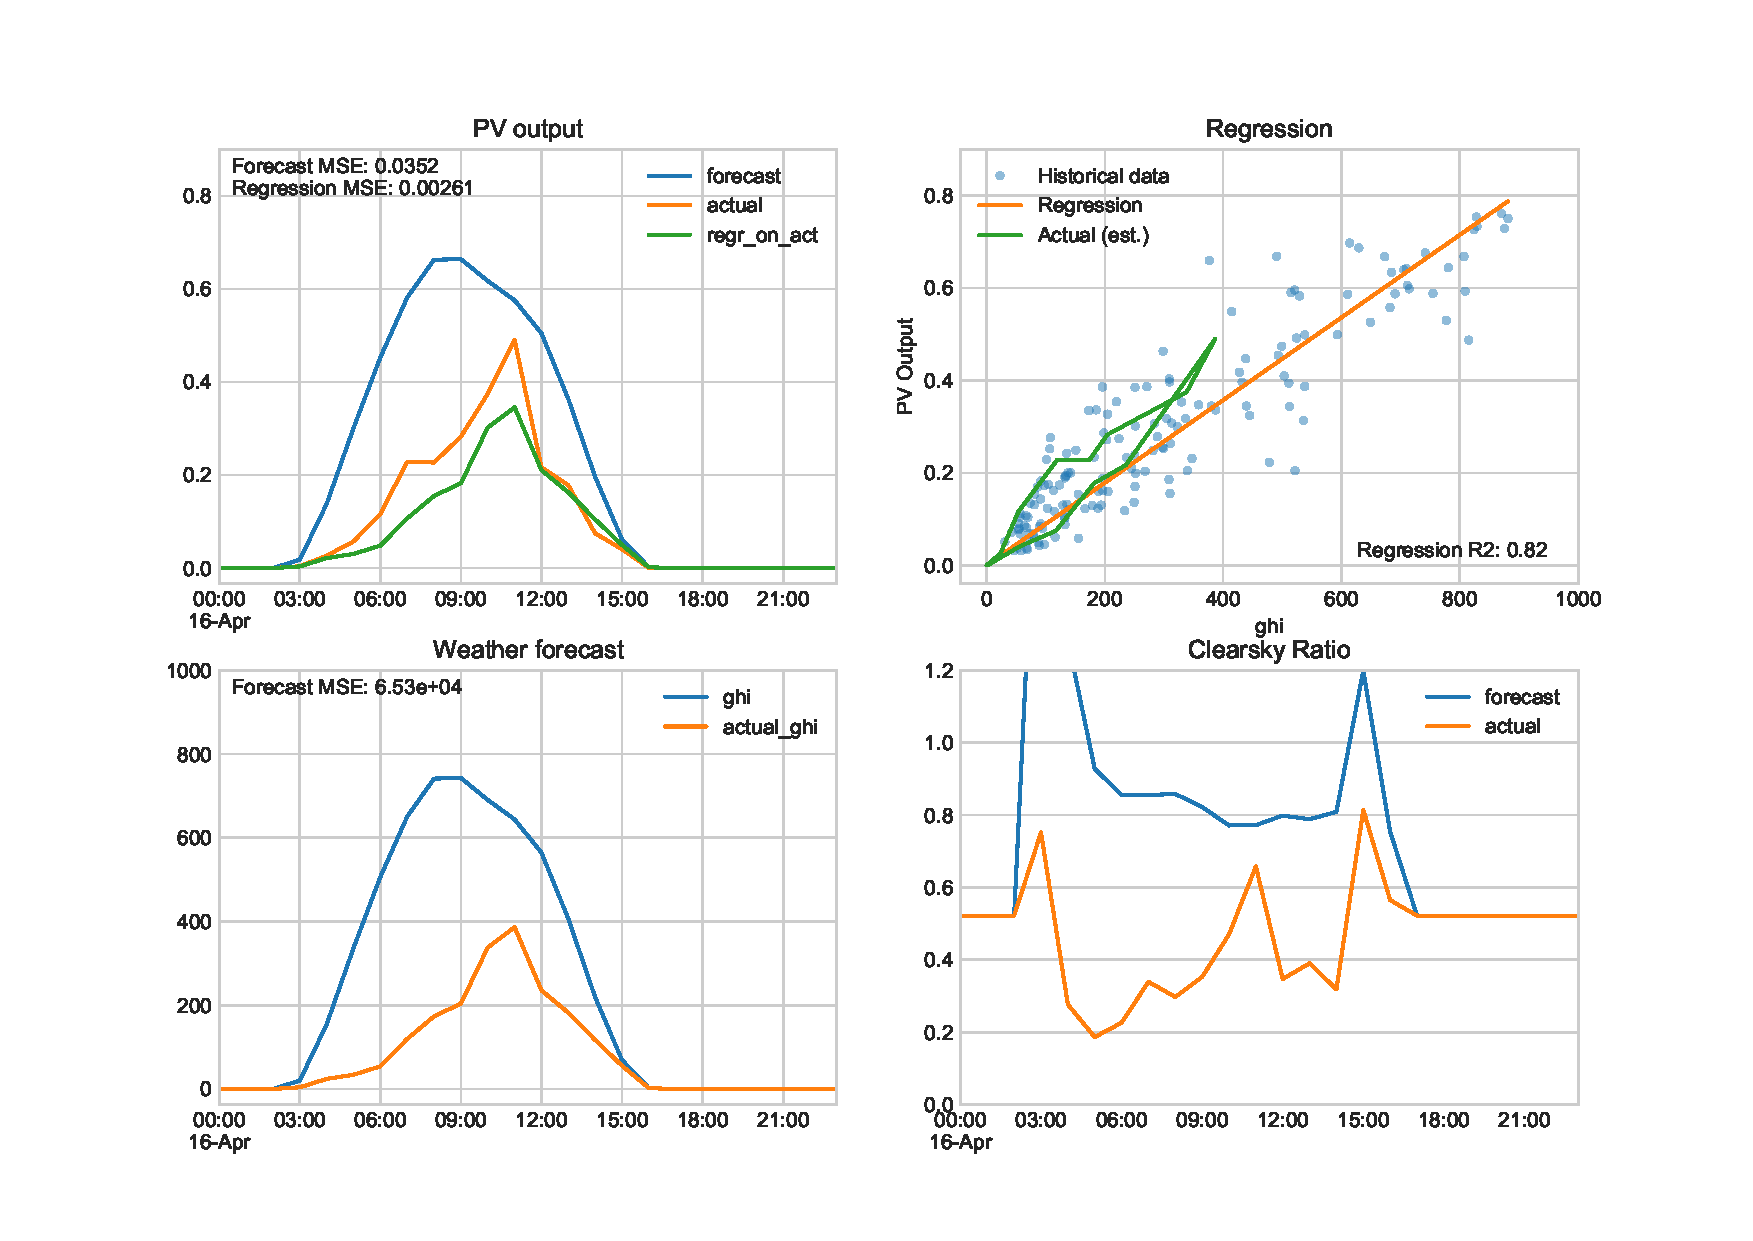
\includegraphics[width=1.0\columnwidth]{SolCastForecasts_w_regr_out_p41.pdf}
	% Convert to png: pdftoppm SolCastForecasts_w_regr_out_p41.pdf SolCastForecasts_w_regr_out_p41 -singlefile -cropbox -png -r 1200
	%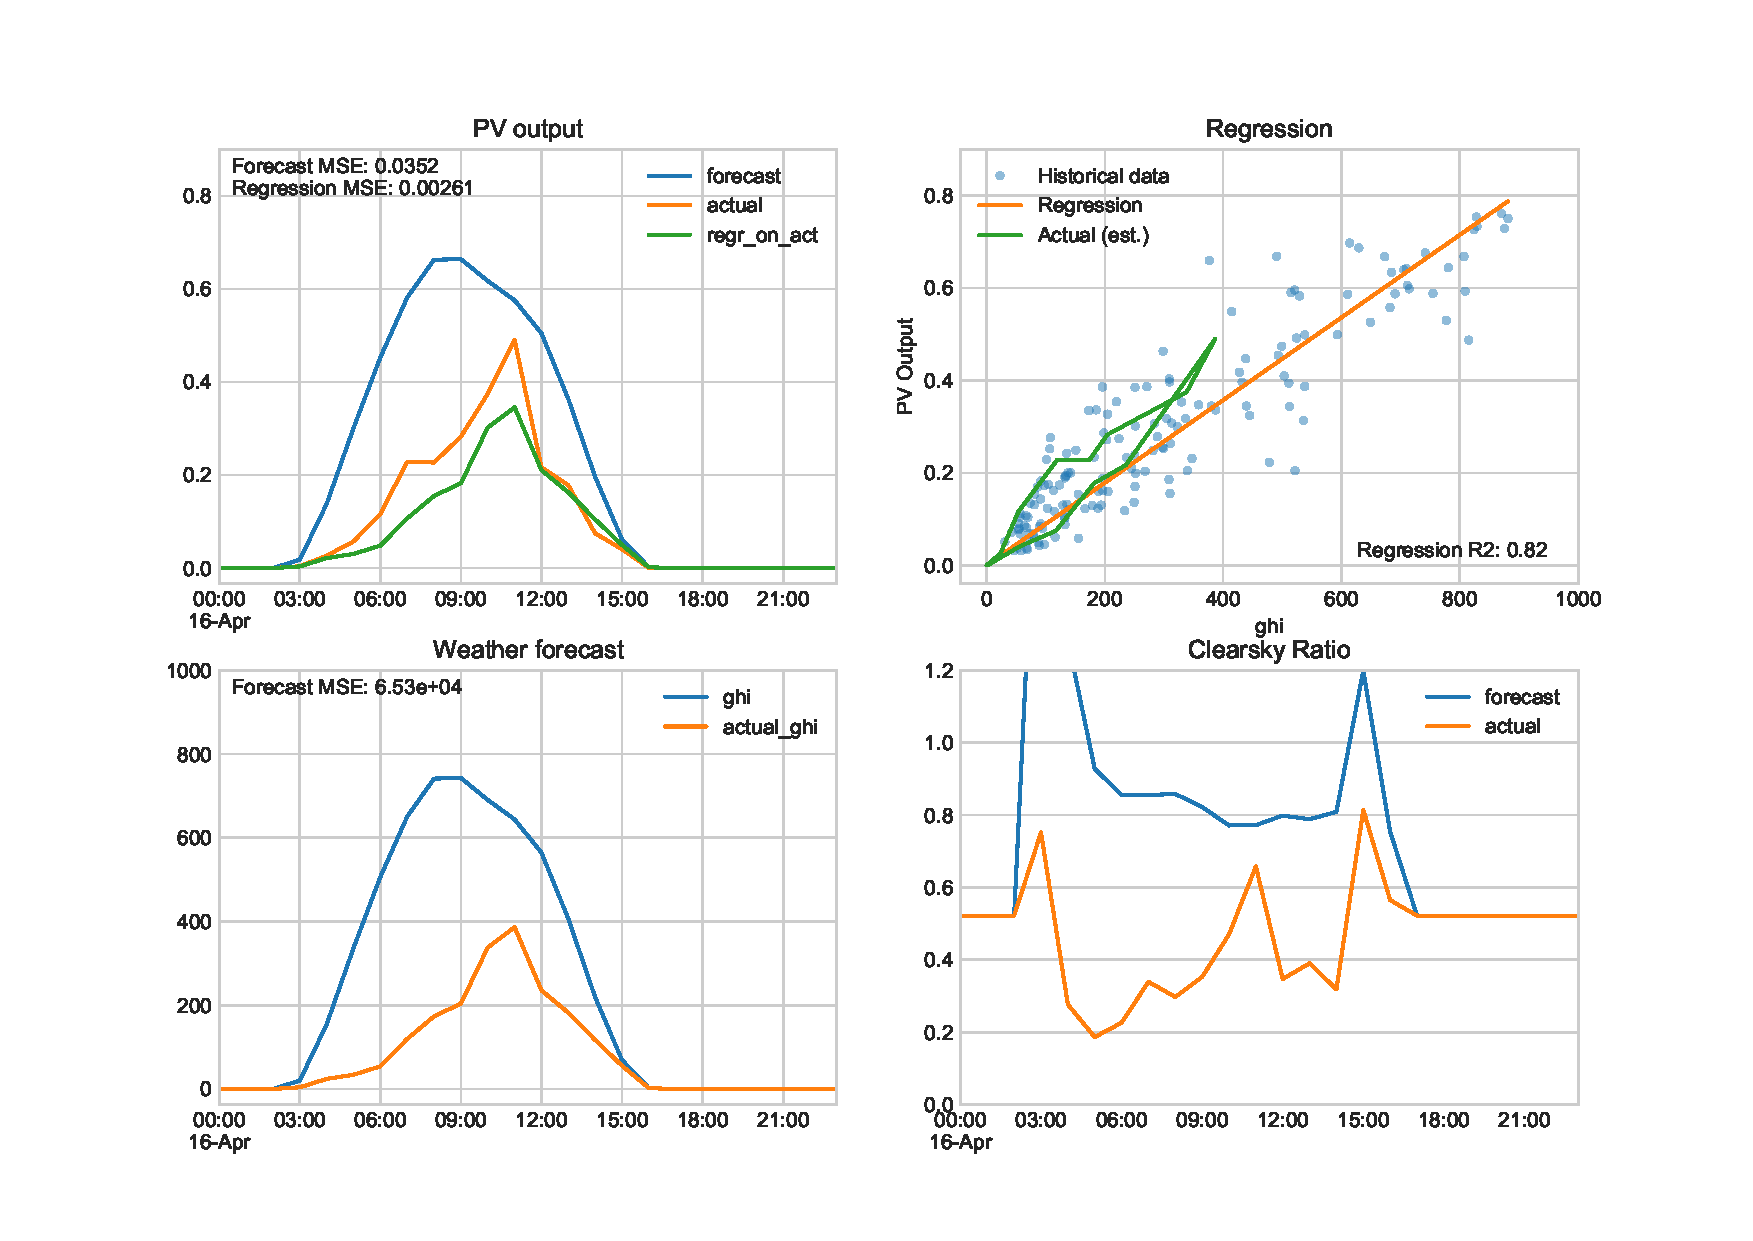
\includegraphics[width=6.5in]{SolCastForecasts_w_regr_out_p41.png}
	\caption{Example Day-ahead Forecast using Solcast Weather Forecast}
	\label{fig:dayahead-forecast-solcast}
\end{figure}


%MeteogramForecasts_cs_ratio  page 41
\begin{figure}[tbh]
	\centering
	% trim=left botm right top
	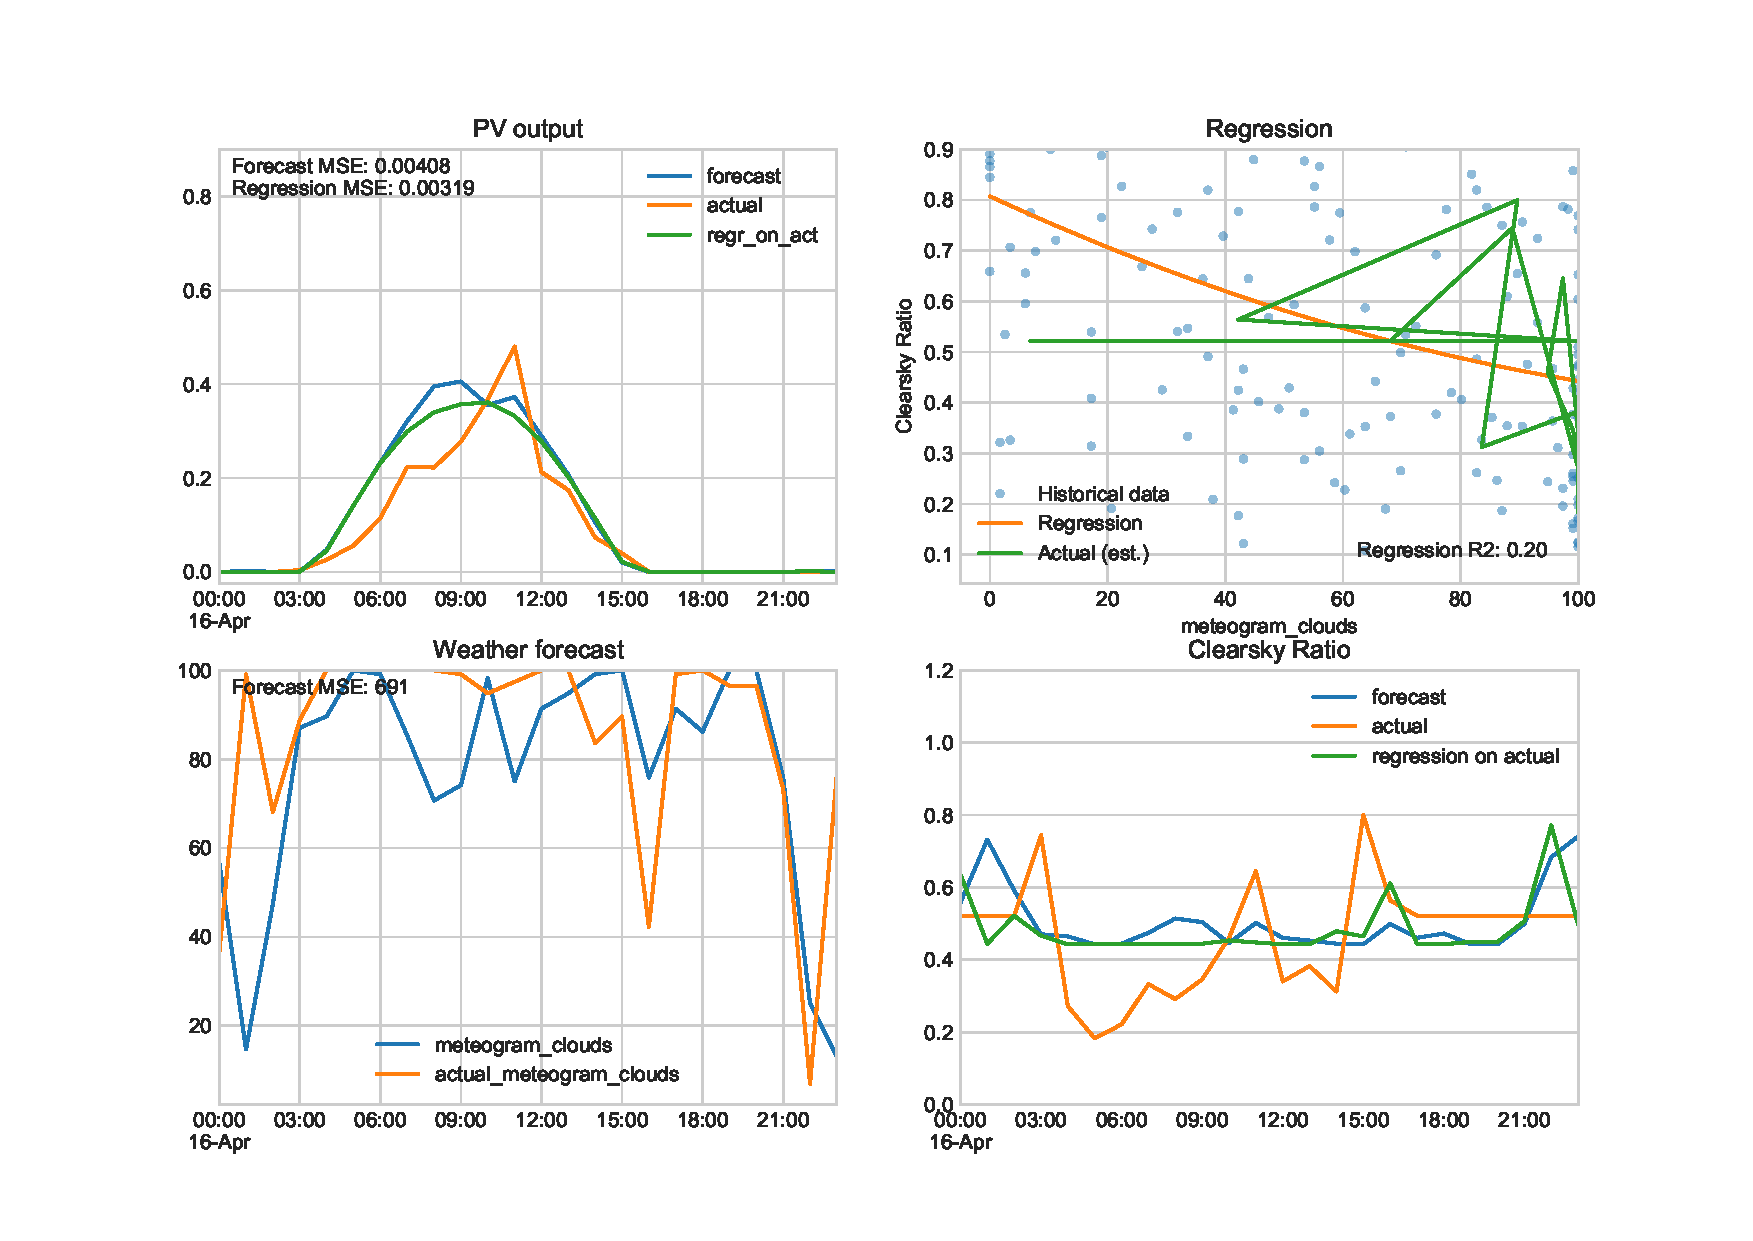
\includegraphics[width=1.0\columnwidth]{MeteogramForecasts_cs_ratio_p41.pdf}
	%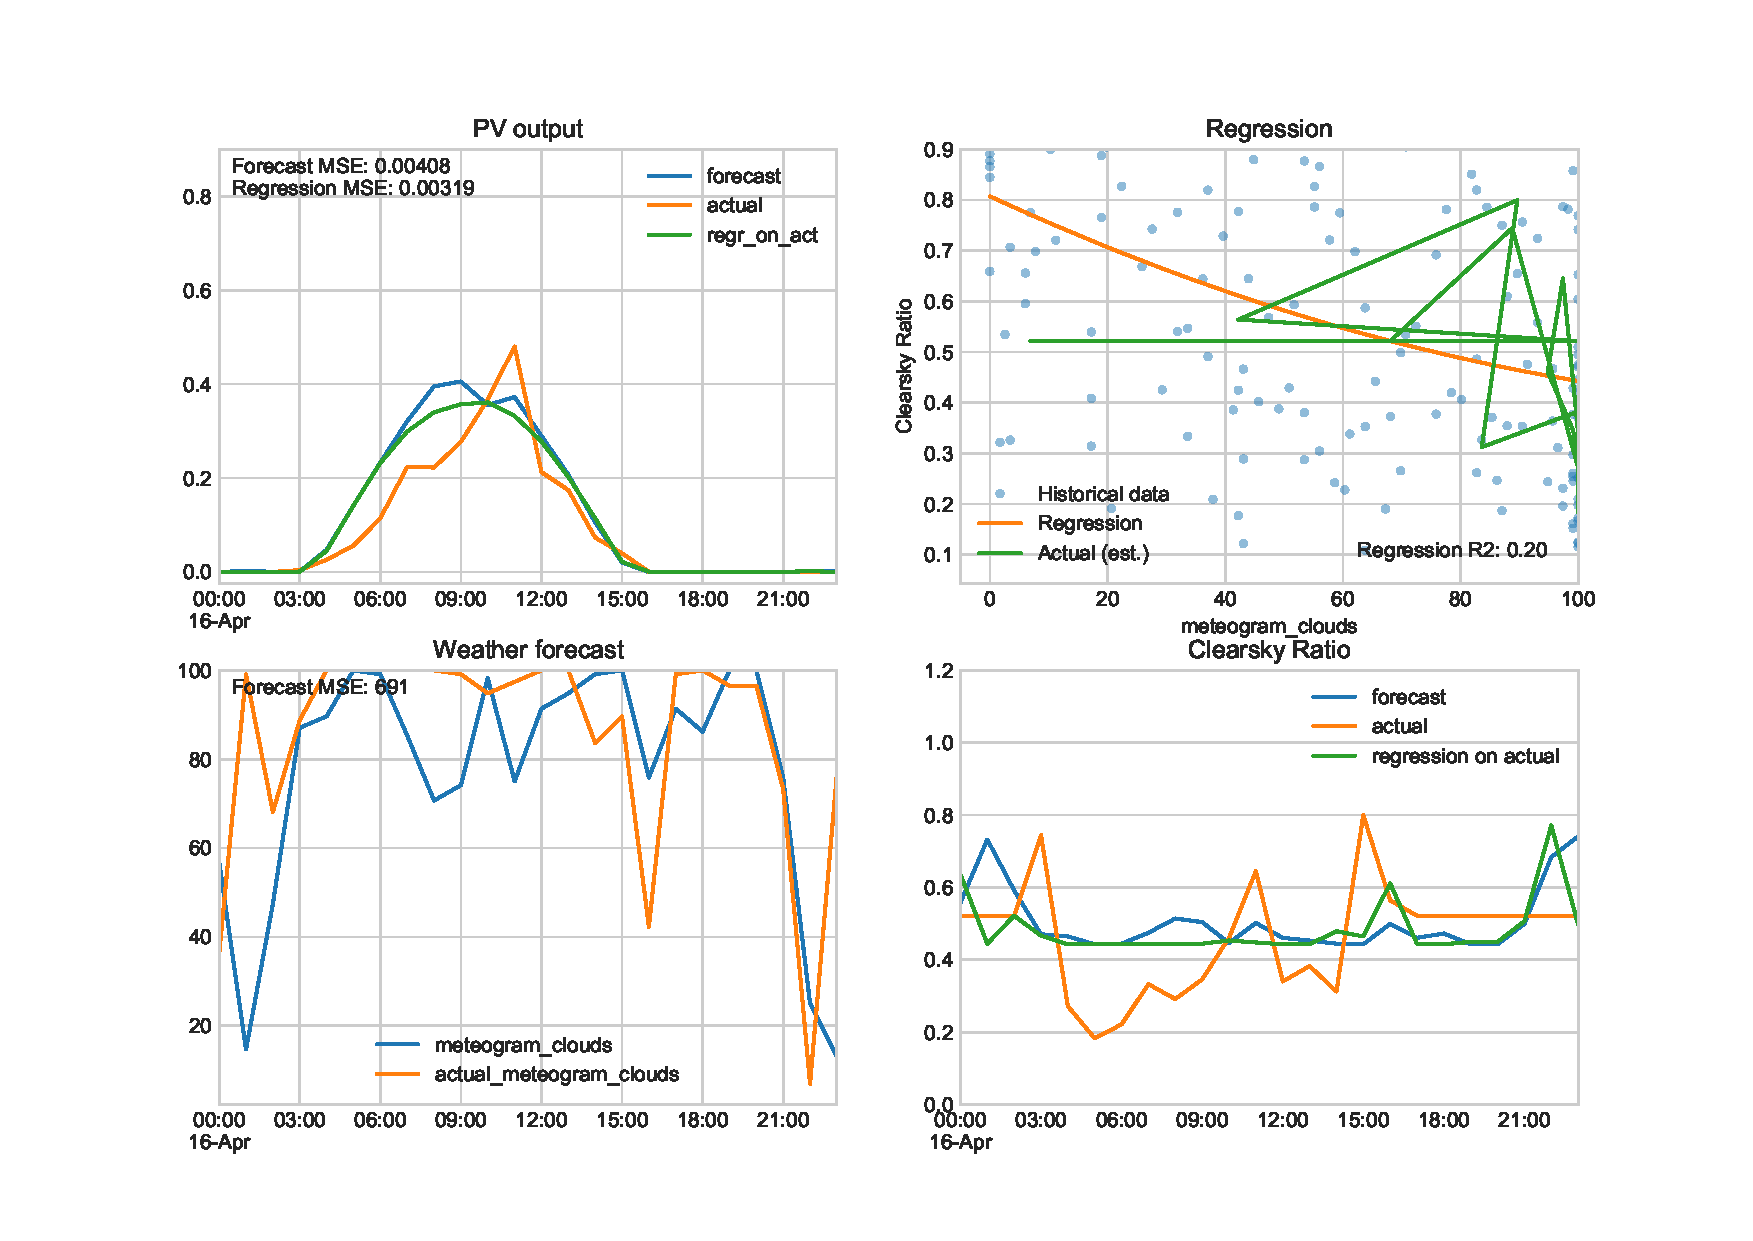
\includegraphics[width=6.5in]{MeteogramForecasts_cs_ratio_p41.png}
	\caption{Example Day-ahead Forecast using MGM Meteogram Weather Forecast}
	\label{fig:dayahead-forecast-meteogram}
\end{figure}


\subsection{Intra-day Updates}

To evaluate and compare the intra-day forecast update methods,
as a starting point, a day-ahead forecast was first generated using the
\pdfmarkupcomment[markup=Highlight,color=yellow]{MGM cloudiness forecast}{Consider changing to the best performing method once results are available}.
This day-ahead forecast was then updated for each hour of the day using each of the methods proposed in \cref{sec:method-intraday}.
In addition to the proposed methods, a reference intra-day update forecast based on persistence was produced.
The persistence forecast was that the clear-sky ratio for the remainder of the day would be the same as the clear-sky ratio from the previous time period.

For comparison, the MSE for the different intra-day forecast update methods was computed for the forecast for one hour, two hours, and six hours ahead.

\begin{figure}[tbh]
	\centering
	% trim=left botm right top
	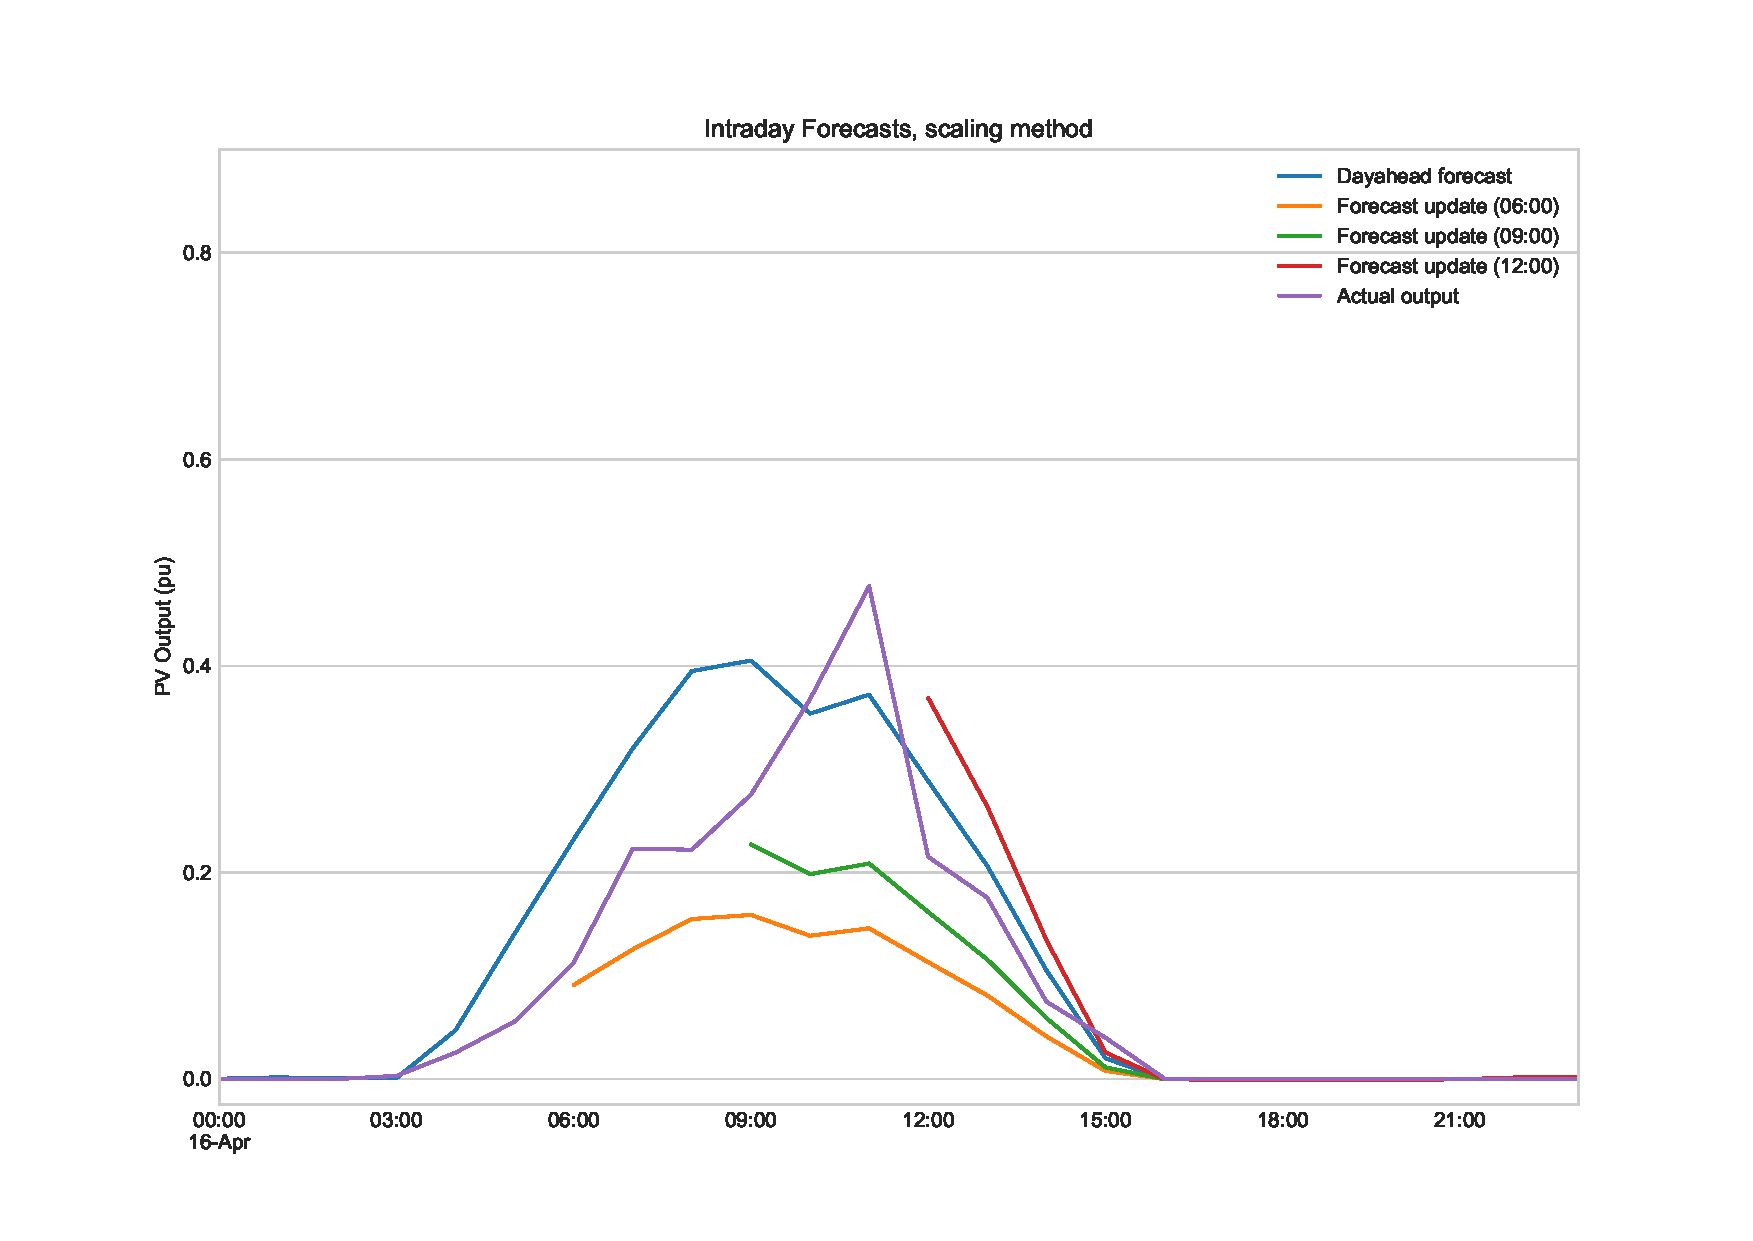
\includegraphics[width=0.85\columnwidth]{Intraday Forecasts_p4.pdf}
	%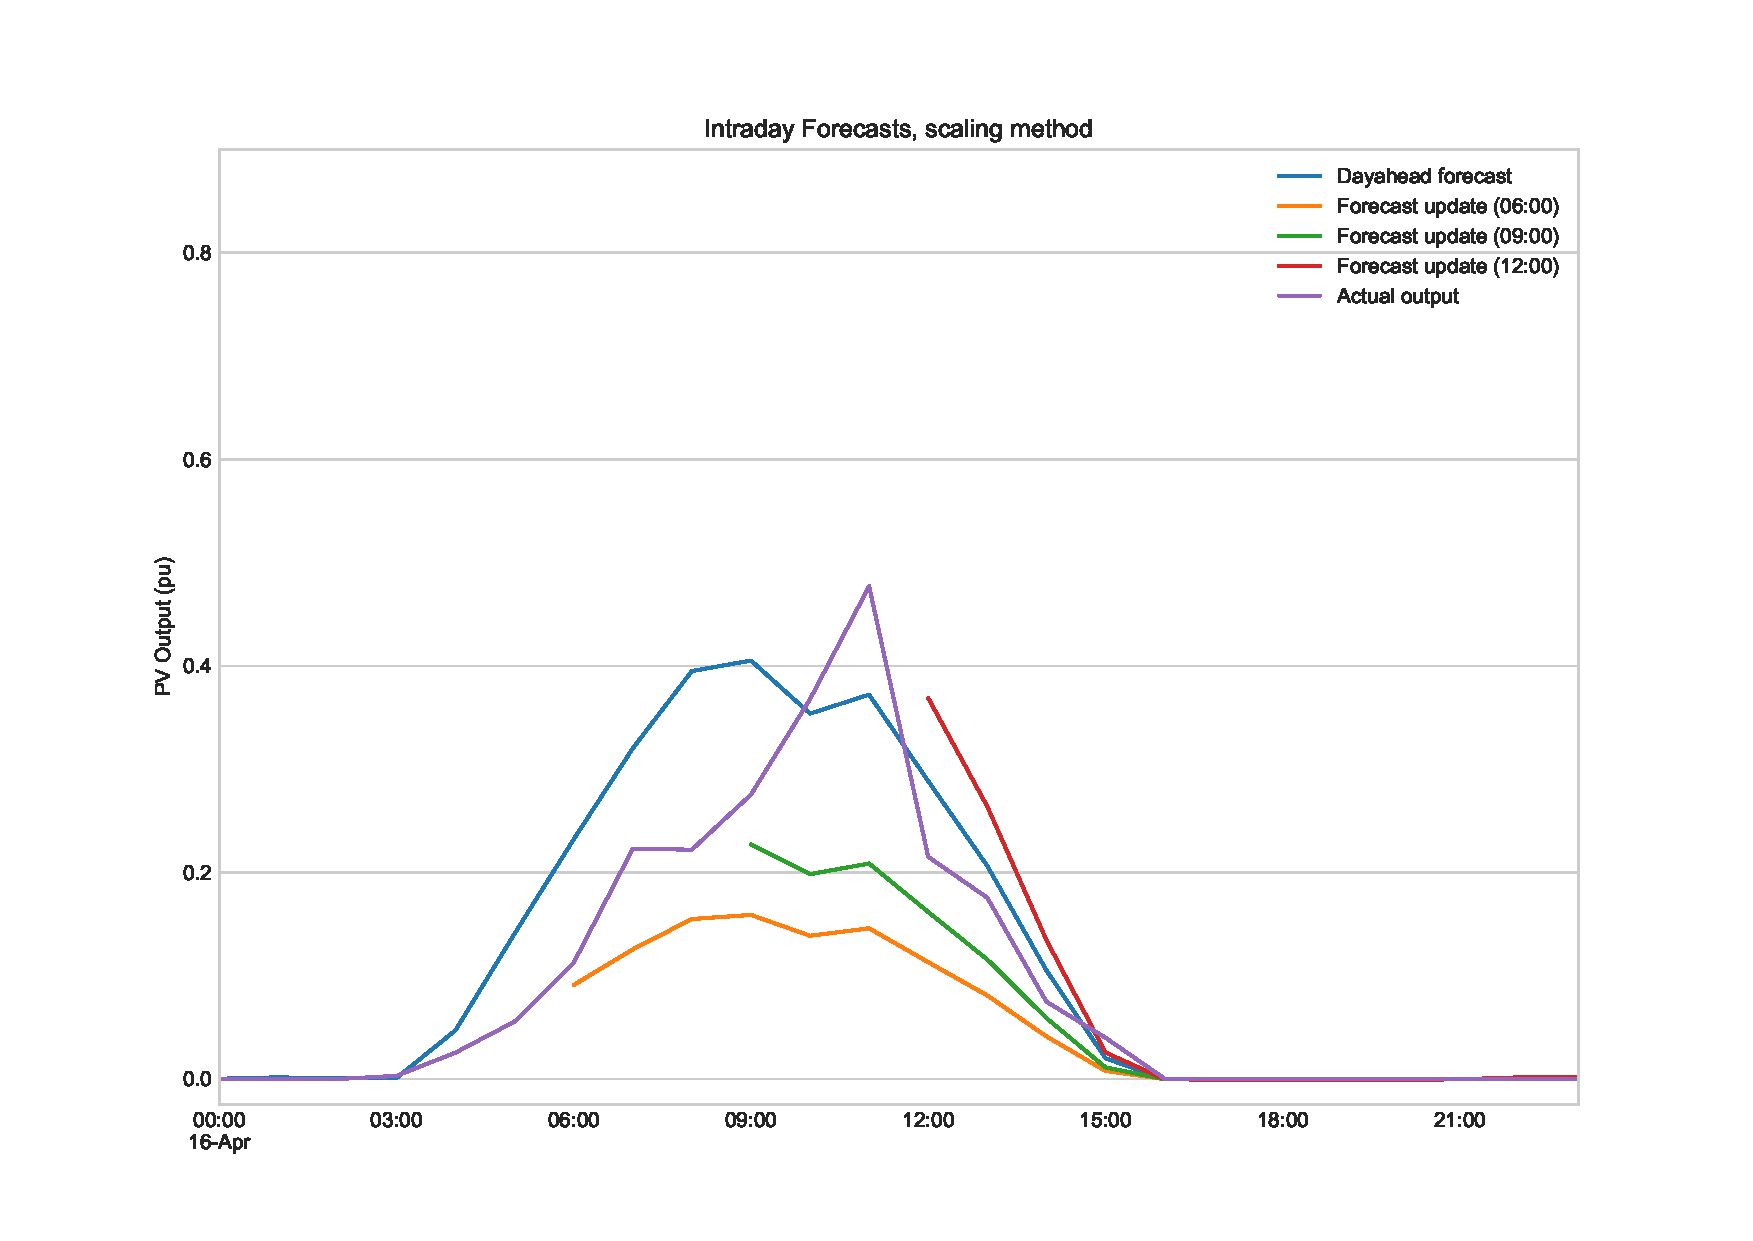
\includegraphics[width=5.53in]{Intraday Forecasts_p4.png}
	\caption{Typical Intra-day Forecasts}
	\label{fig:intraday-forecast}
\end{figure}


\subsection{Optimal Energy Dispatch}

To demonstrate the effectiveness of the developed methods in the target application,
the forecasts were input into an agricultural microgrid operational optimization and simulation program.
The optimization formulation was previously presented in \cite{Brown2022}.
The use of model-predictive control was simulated by using the optimizer to choose the optimal ratio of using excess available PV energy between energy storage in a battery energy storage system (BSS) and utilization to pump water into a reservoir.
The MPC optimization was performed using the forecast PV data, including intra-day updates.
The operation for the following period was then simulated using actual PV data.
A flowchart of the MPC simulation is shown in \cref{fig:mpc-simulation-flowchart}.

% Figure copied from last progress report
\begin{figure}[tbh]
	\centering
	% trim=left botm right top
	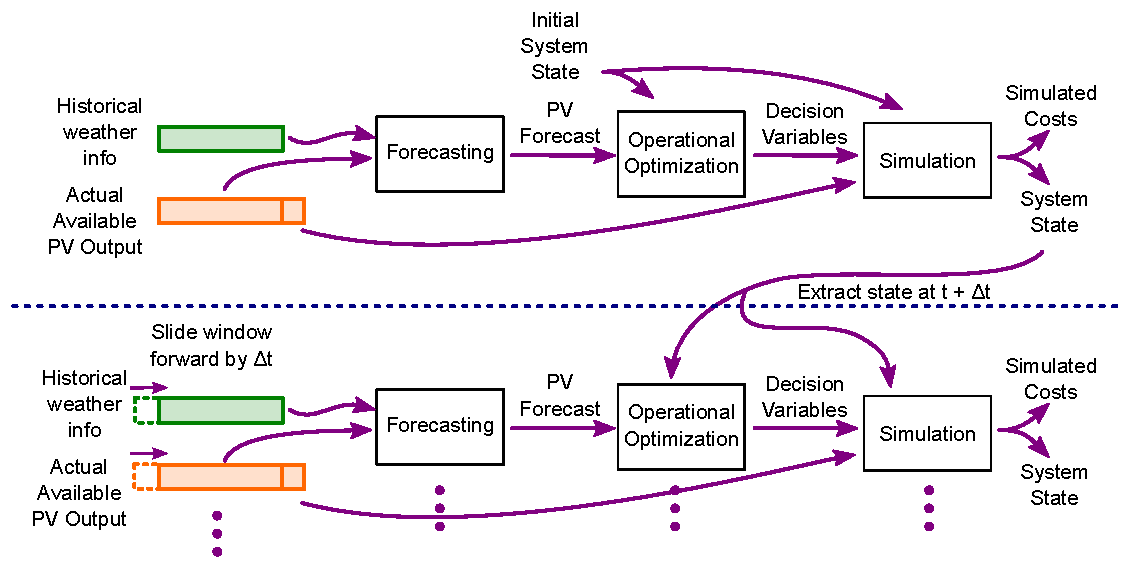
\includegraphics[width=1.0\columnwidth]{MPC Demo System Diagram.pdf}
	\caption{MPC demonstration simulation flowchart}
	\label{fig:mpc-simulation-flowchart}
\end{figure}

